\chapter{El cálculo de Newton del número pi}

\section{La revolución matemática de 1666}

\noindent \textbf{SIMPLICIO:} He oído que Newton tenía una forma muy
ingeniosa de calcular $\pi$. ¿Podría hablarme de ello?

\noindent \textbf{SÓCRATES:} Por supuesto. Todo empieza alrededor de
1665-1666, cuando Newton estaba a punto de cumplir 23 años. ¿Recuerdas
algo significativo sobre ese año?

\noindent \textbf{SIMPLICIO:} ¿No es ese el \textit{``annus mirabilis''}
de Newton, su año de los milagros? Si mal no recuerdo, se vio obligado a
abandonar Cambridge debido a un brote de la Gran Peste, y realizó sus
descubrimientos más trascendentales (cálculo, óptica, gravitación, etc.)
mientras guardaba cuarentena en aislamiento en su casa familiar de
Woolsthorpe.

\noindent \textbf{SÓCRATES:} Exactamente. Y una de las primeras cosas
que descubrió en ese año fue una nueva versión del teorema del
binomio. Dime, por favor, ¿qué se puede decir sobre $(1 + x)^n$?

\noindent \textbf{SIMPLICIO:} Claro, si desarrollas $(1 + x)^n$, obtienes:
\[ \binom{n}{0} + \binom{n}{1}x + \binom{n}{2}x^2 + \dots + \binom{n}{n}x^n \]
\noindent Aquí $\binom{n}{k}$ es el ``coeficiente binomial'', el número
de formas de elegir $k$ objetos de un conjunto de $n$. Explícitamente,
$\binom{n}{k} = \frac{n!}{k!(n-k)!}$. Estos son simplemente los números
del triángulo de Pascal, y puedes leer fácilmente la fila $n$-ésima.

\begin{center}
    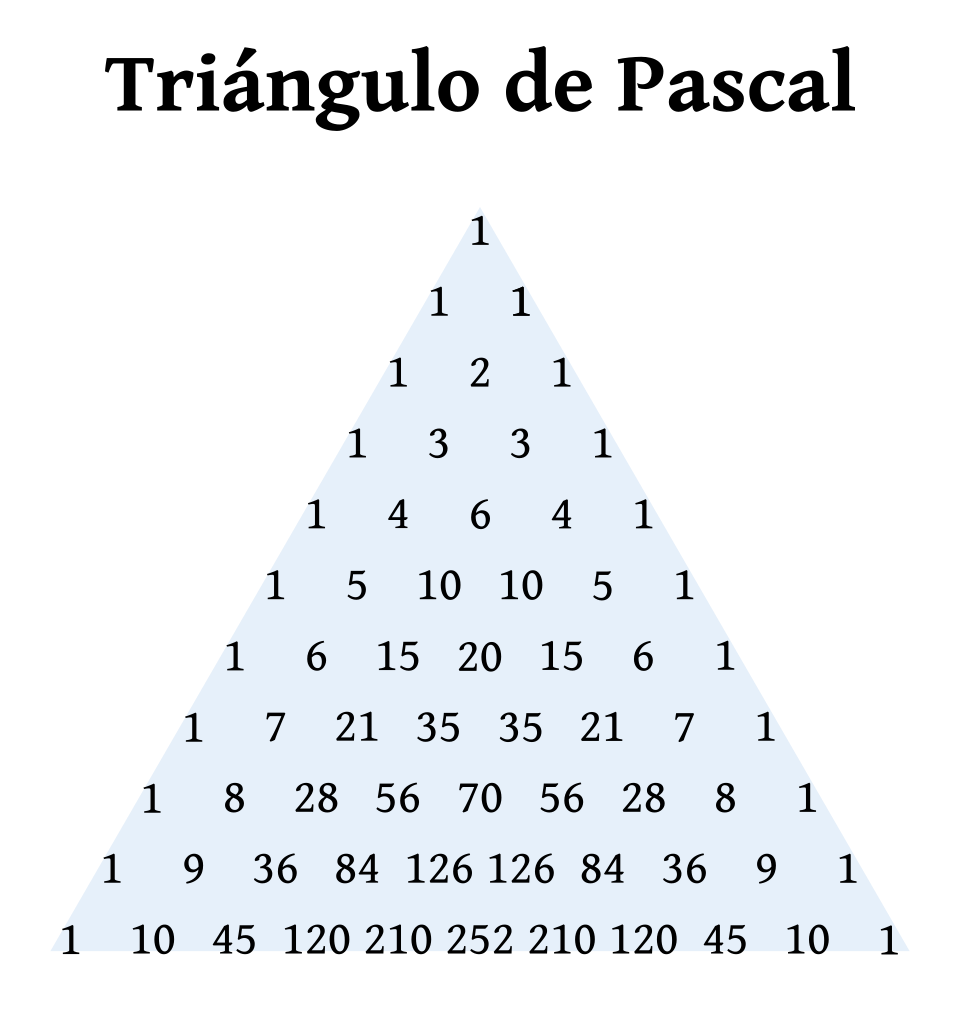
\includegraphics[width=0.5\linewidth]{fig/Triangulo_de_Pascal.png}
\end{center}

\noindent \textbf{SÓCRATES:} ¡Excelente! ¿Y conoces la notación sigma?

\noindent \textbf{SIMPLICIO:} Creo que sí. Podría haber escrito lo mismo
como $\sum_{k=0}^{n} \binom{n}{k} x^k$. En general, si tienes una función
$f : \mathbb{N} \to \mathbb{R}$ y quieres expresar
$f(a) + f(a + 1) + \dots + f(b)$, es decir, la suma de $f(k)$ mientras
$k$ varía desde un entero $a$ hasta otro entero $b$, puedes escribirlo
como $\sum_{k=a}^{b} f(k)$.

\noindent \textbf{SÓCRATES:} Muy bien. Así que tenemos
$(1 + x)^n = \sum_{k=0}^{n} \binom{n}{k} x^k$. Ahora, ¿me permitirías
escribir esto como una suma que llegue hasta el infinito?
\[ (1 + x)^n = \sum_{k=0}^{\infty} \binom{n}{k} x^k \]

\noindent \textbf{SIMPLICIO:} Hmm. Vale, creo que entiendo a qué te
refieres: el triángulo de Pascal tiene ceros implícitos en todas partes
por fuera, así que $\binom{n}{k}$ es simplemente cero en cuanto $k >
n$. Así que lo has escrito como una suma infinita, aunque secretamente
termina tras un número finito de términos. Pero, ¿para qué sirve
extenderla así?

\noindent \textbf{SÓCRATES:} Bueno, déjame preguntarte esto: ¿se te
ocurre alguna forma de dar sentido a esta fórmula cuando $n = -1$?

\noindent \textbf{SIMPLICIO:} ¡¿Cómo?! No puedes usar coeficientes
binomiales. ¡¿Cómo vas a elegir 3 cosas de un conjunto de $-1$?! ¡Eso no
tiene sentido!

\noindent \textbf{SÓCRATES:} Tienes razón, pero muchos de los grandes
descubrimientos en matemáticas ocurren cuando te das cuenta de que
puedes ``romper las reglas'' y seguir un patrón más allá de su límite
previsto. Ponte en el lugar de Newton; ¿qué se le ocurriría a un genio
como él?

\noindent \textbf{SIMPLICIO:} Bueno, tenemos esta otra fórmula para los
coeficientes binomiales, no en términos combinatorios, sino con
factoriales: $\binom{n}{k} = \frac{n!}{k!(n-k)!}$. Eso sigue sin ayudar
porque, ¡¿qué demonios se supone que es $(-1)!$?! ¡Ah, espera! También
podemos escribirlo así:
\[ \binom{n}{k} = \frac{n(n - 1)(n - 2) \dots (n - k + 1)}{k!} \] Y de
esta manera, ``esquivamos'' el problema de lidiar con $(-1)!$ y pasamos
directamente a números ``normales''.

\noindent \textbf{SÓCRATES:} ¿Podrías escribir esto usando la notación
de productorio?

\noindent \textbf{SIMPLICIO:} Claro, es como la notación de sumatorio
pero con una $\Pi$:
\[ \binom{n}{k} = \frac{1}{k!} \prod_{\ell=1}^{k} (n - \ell) \]

\noindent \textbf{SÓCRATES:} ¡Vaya! ¿Estás seguro de los límites de ese
producto?

\noindent \textbf{SIMPLICIO:} ¡Argh! Es tan fácil cometer un error
tonto. Después de escribir la fórmula, debería haber comprobado que los
valores de inicio y fin fueran correctos; el contador $\ell$ debería ir de
$0$ a $k - 1$, no de $1$ a $k$. ¿Así mejor?
\[ \binom{n}{k} = \frac{1}{k!} \prod_{\ell=0}^{k-1} (n - \ell) \]

\noindent \textbf{SÓCRATES:} Perfecto. Continúa.

\noindent \textbf{SIMPLICIO:} Vale, si aceptamos seguir este patrón,
obtenemos:
\begin{itemize}
\item $\binom{-1}{0} = 1$, lo cual tiene sentido porque cualquier fila
  del triángulo de Pascal empieza por $1 = \binom{c}{0}$.
\item $\binom{-1}{1} = (-1)/1! = -1$, que también tiene sentido porque
  el siguiente término en la ``fila $c$'' es siempre $\binom{c}{1} = c$.
\item $\binom{-1}{2} = (-1)(-2)/2! = +1$.
\item $\binom{-1}{3} = (-1)(-2)(-3)/3! = -1$.
\end{itemize}
Ya veo el patrón: simplemente alterna entre $+1$ y $-1$, así que la
serie queda:
\[ (1 + x)^{-1} = 1 - x + x^2 - x^3 + x^4 - x^5 + \dots \]

\noindent \textbf{SÓCRATES:} ¡Muy bien! Pero, ¿tiene esta fórmula algún
sentido real? ¿Cómo podrías ponerla a prueba?

\noindent \textbf{SIMPLICIO:} Vale, si se supone que esa serie
``representa'' a $1/(1 + x)$, entonces si multiplico todo por $(1 + x)$,
debería obtener simplemente $1$. Vamos a probar:
\[ (1 + x)(1 - x + x^2 - x^3 + x^4 - x^5 + \dots) = ? \]
Primero multiplicaré todo por $1$, luego por $x$, y los sumaré.
\[ (1 - x + x^2 - x^3 + x^4 - x^5 + \dots) + (x - x^2 + x^3 - x^4 + x^5 \dots) \]
Si reordeno los términos, todo se cancela y solo queda el $1$
inicial. ¡Genial!

\noindent \textbf{SÓCRATES:} Interesante. ¿Y se te ``permite'' reordenar
los términos así?

\noindent \textbf{SIMPLICIO:} Bueno... ¿por qué no?

\noindent \textbf{SÓCRATES:} Olvídalo por ahora; pareces satisfecho con
que tenga sentido decir que la serie
$1 - x + x^2 - x^3 + x^4 - x^5 + \dots$ ``converge'' (sea lo que sea que
eso signifique) a $(1 + x)^{-1}$.

\noindent \textbf{SIMPLICIO:} Pensándolo bien, ya sabía esto; ¡es solo
la serie geométrica! Sé que
$1 + \lambda + \lambda^2 + \lambda^3 + \dots$ suma $1/(1 - \lambda)$, y nuestra serie
simplemente reemplaza $\lambda$ por $-x$.

\noindent \textbf{SÓCRATES:} Sí, muy bien. ¿Y dónde podría ``encajar''
esto en el triángulo de Pascal?

\noindent \textbf{SIMPLICIO:} ¡Cielos! ¿Acabamos de descubrir una
extensión del triángulo que va hacia ``arriba''?

\begin{center}
    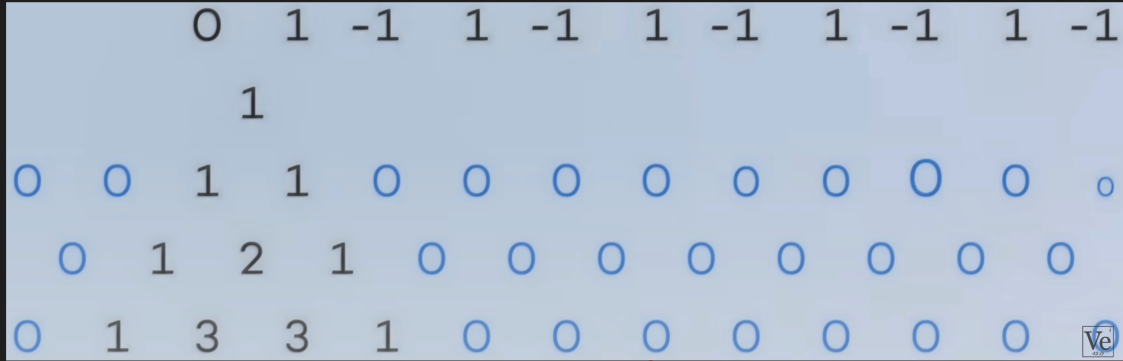
\includegraphics[width=0.5\linewidth]{fig/Triangulo_de_Pascal_arriba.png}
\end{center}

\noindent \textbf{SÓCRATES:} En efecto, y de hecho podemos continuar
este patrón para $n = -2, -3, -4$, y así sucesivamente. Te dejaré que lo
deduzcas tú mismo, ¡pero en realidad obtenemos todo otro Triángulo de
Pascal (con algunos signos negativos) por encima del estándar!

\begin{center}
    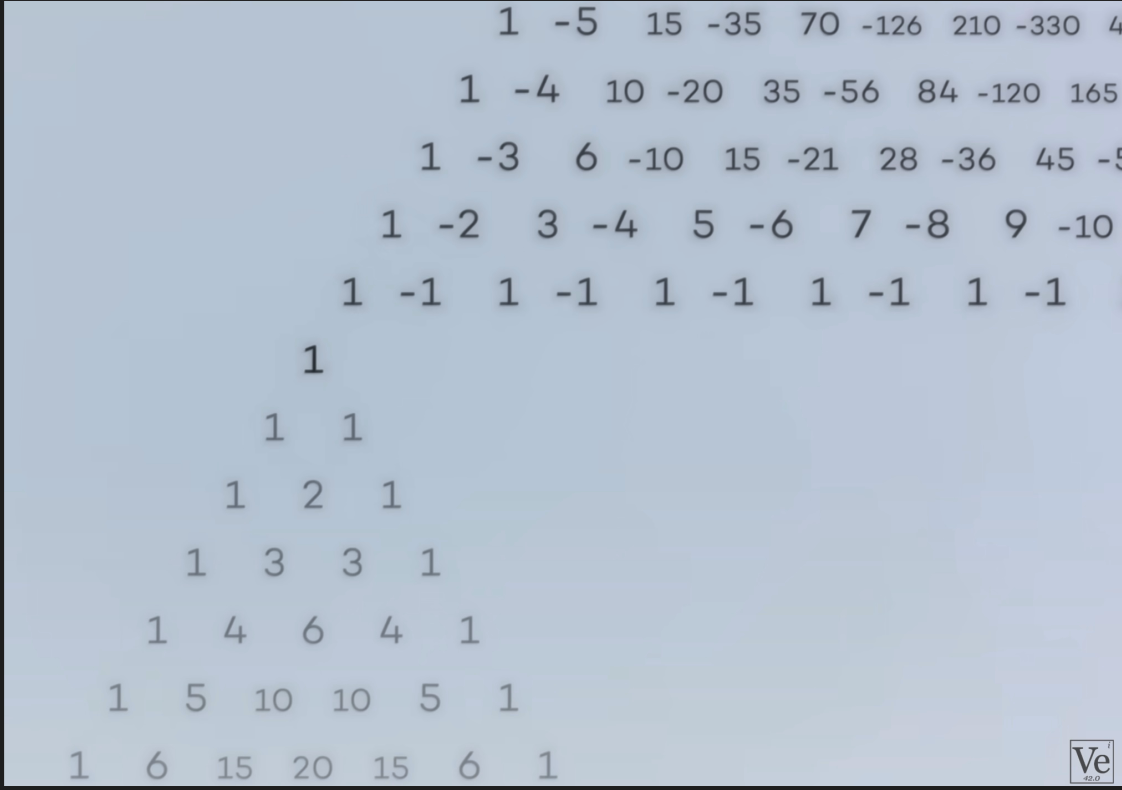
\includegraphics[width=0.5\linewidth]{fig/Triangulo_de_Pascal_extendido.png}
\end{center}

\noindent ¿Ves cómo sigue cumpliendo la regla habitual de que los dos
números de arriba sumen el valor que tienen justo debajo? Pero probemos
algo aún más exótico. ¿Puedes hacer que el Teorema del Binomio funcione
para $n = 1/2$?

\noindent \textbf{SIMPLICIO:} ¡Hala! ¿$n = 1/2$? Eso es... ¡forzar mucho
las cosas! Pero déjame intentar usar la misma fórmula. Así que
$\binom{1/2}{k} = \frac{1}{k!} \prod_{\ell=0}^{k-1} (1/2 - \ell)$. Voy a calcular
los primeros términos:
\begin{itemize}
\item $\binom{1/2}{0} = 1$ (como siempre).
\item $\binom{1/2}{1} = (1/2)/1! = 1/2$ (de nuevo, coincide con el
  patrón que ya conocíamos).
\item $\binom{1/2}{2} = (1/2)(-1/2)/2! = -1/8$.
\item $\binom{1/2}{3} = (1/2)(-1/2)(-3/2)/3! = 1/16$.
\item $\binom{1/2}{4} = \frac{(1/2)(-1/2)(-3/2)(-5/2)}{4!} = -5/128$.
\end{itemize}
Así que $(1 + x)^{1/2} = 1 + \frac{1}{2}x - \frac{1}{8}x^2 + \frac{1}{16}x^3 - \frac{5}{128}x^4 + \dots$\\
Pero espera... ¡¿se supone que esto es $\sqrt{1 + x}$?!

\noindent \textbf{SÓCRATES:} De nuevo, entra en la mente de Newton:
¿cómo podría él justificar si esta fórmula tiene algún sentido?

\noindent \textbf{SIMPLICIO:} ¡Ah, ya veo! Si elevamos la fórmula al
cuadrado y lo multiplicamos todo, supongo que deberíamos obtener
$1 + x$; eso justificaría llamar a la serie $\sqrt{1 + x}$.

\noindent \textbf{SÓCRATES:} ¡Adelante!

\noindent \textbf{SIMPLICIO:} Vale, quiero calcular:
\[ \left( 1 + \frac{1}{2}x - \frac{1}{8}x^2 + \frac{1}{16}x^3 - \frac{5}{128}x^4 + \dots \right)^2 \]
Eso significa elevar cada término al cuadrado, y también añadir el doble
de cada producto de pares distintos de términos.

\noindent \textbf{SÓCRATES:} Correcto. ¿Se te ocurre una buena forma de
llevar la cuenta de todo?

\noindent \textbf{SIMPLICIO:} ¡Oh, ya sé! Vamos a agrupar las cosas por
la potencia de $x$ involucrada. La primera es fácil: $x^0 = 1$, que solo
se obtiene elevando al cuadrado el primer término. Así que ese
coeficiente es $1$.
\\
Para el coeficiente de $x^1$, no puedo elevar al cuadrado nada que
contenga $x$, así que solo puedo multiplicar el término en $x$ por el
término constante y, por supuesto, duplicarlo. Eso es simplemente
$2 \times 1 \times \frac{1}{2}x = x$. Así que el coeficiente de $x$ es $1$.
\\
Para $x^2$, obtengo dos contribuciones: de constante por cuadrático,
$2 \times 1 \times (-\frac{1}{8}x^2) = -\frac{1}{4}x^2$, y también del cuadrado
del término lineal: $(\frac{1}{2}x)^2 = \frac{1}{4}x^2$. Así que el
coeficiente total es $-\frac{1}{4} + \frac{1}{4} = 0$.
\\
Probemos unos pocos más. Para obtener $x^3$, necesito:
\begin{itemize}
    \item $2 \times 1 \times \frac{1}{16}x^3 = \frac{1}{8}x^3$ (constante por el término $x^3$)
    \item $2 \times \frac{1}{2}x \times (-\frac{1}{8}x^2) = -\frac{1}{8}x^3$ (el término $x$ por el término $x^2$)
\end{itemize}
Así que el coeficiente total de $x^3$ es $\frac{1}{8} - \frac{1}{8} = 0$.
\\
¡Esto es increíble! Parece que todos los términos de orden superior se
cancelan perfectamente. Apuesto a que eso seguirá pasando y el cuadrado
resultará ser exactamente $1 + x$; ¡la fórmula realmente funciona!
\\
Pero espera, ¡¿ahora tenemos otra fila entera en el triángulo de Pascal,
entre las filas 0 y 1?!

\begin{center}
    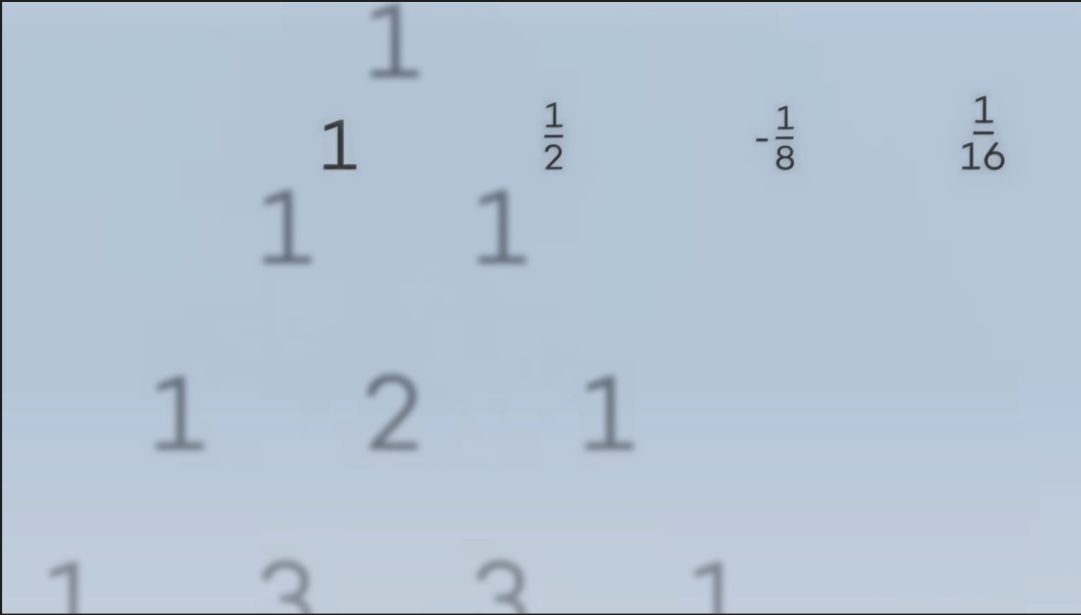
\includegraphics[width=0.5\linewidth]{fig/Triangulo_de_Pascal_racional.png}
\end{center}

\noindent \textbf{SÓCRATES:} Hermoso, ¿verdad?

\noindent \textbf{SIMPLICIO:} Espera, esto es mucho más sencillo de lo
que parece. ¿No es esto simplemente lo mismo que el desarrollo de Taylor
alrededor de $x = 0$ de la función $f(x) = \sqrt{1 + x}$? Ya sé cómo
hacer eso por mis clases de Cálculo.

\noindent \textbf{SÓCRATES:} Sí, muy bien; pero Brook Taylor (el de las
series de Taylor) no demostró su teorema general hasta 1715, unas
décadas después del cálculo de $\pi$ de Newton.

\noindent \textbf{SÓCRATES:} Ahora, supón que quisieras calcular algo
como $\sqrt{3}$. ¿Se te ocurre alguna forma de hacerlo usando esta
fórmula?

\noindent \textbf{SIMPLICIO:} Hmm, la función es $\sqrt{1 + x}$, así que
supongo que quiero poner $x = 2$. Entonces obtengo:
\[ \sqrt{1 + 2} = 1 + \frac{1}{2}2 - \frac{1}{8}2^2 + \frac{1}{16}2^3 - \frac{5}{128}2^4 + \dots \]
Sumar estos cinco términos da $11/8 = 1,375$, que no está muy cerca de
$\sqrt{3} \approx 1,73$. Además, los términos individuales no son tan
pequeños; por ejemplo, el último es $\frac{5}{128}2^4 = 5/8 = 0,625$.

\noindent \textbf{SÓCRATES:} Bueno, claro, si eliges una $x$ grande,
como $x > 1$, entonces las potencias de $x$ son cada vez más grandes (¡y
exponencialmente!). ¿Se te ocurre alguna otra cosa que pudieras hacer?

\noindent \textbf{SIMPLICIO:} ¡Ah, ya veo! Sé que $3$ está cerca de $4$,
que es un cuadrado perfecto. ¿Y si escribimos:
\[ \sqrt{3} = \sqrt{4 - 1} = \sqrt{4(1 - 1/4)} = 2\sqrt{1 - 1/4} \]
Así que ahora, si aplico nuestra fórmula con $x = -1/4$ (¡que es menor
que uno!), supongo que obtendré:
\[ \sqrt{3} \approx 2 \left( 1 + \frac{1}{2}(-1/4) - \frac{1}{8}(-1/4)^2 + \frac{1}{16}(-1/4)^3 - \frac{5}{128}(-1/4)^4 + \dots \right) \]
Tomando solo estos cinco términos, la fracción de la derecha sale
$28379/16384 \approx 1,73212$, que es impresionantemente cercana a $\sqrt{3} \approx
1,7320508$. ¡Hemos obtenido 3 decimales de precisión, nada mal!

\noindent \textbf{SÓCRATES:} ¡Genial! Ahora ves el poder del teorema del
binomio de Newton. Vale, volvamos entonces a tu pregunta original sobre
la estimación de $\pi$ de Newton.

\noindent \textbf{SIMPLICIO:} Hmmm, $\pi$ es la relación entre la
circunferencia y el diámetro de un círculo. Pero, ¿de dónde voy a sacar
una longitud?

\noindent \textbf{SÓCRATES:} ¡Ah! Pero, ¿qué aprendimos de Arquímedes?

\noindent \textbf{SIMPLICIO:} ¡Oh! Que $\pi$ también es un \textit{área},
no solo una longitud. Es el área de un círculo unidad $\pi r^2$ donde
$r = 1$.

\noindent \textbf{SÓCRATES:} Precioso. ¿Y podrías encontrar el área de
un círculo escondida en alguna parte?

\noindent \textbf{SIMPLICIO:} ¡Creo que lo veo! Gracias a Descartes y a
las coordenadas ``cartesianas'', podemos expresar el círculo como la
gráfica de $x^2 + y^2 = 1$, o para convertirlo en una función,
$y = \sqrt{1 - x^2}$. Así que solo tenemos que reemplazar $x$ en nuestra
serie por $-x^2$.
\[ \sqrt{1 - x^2} = 1 + \frac{1}{2}(-x^2) - \frac{1}{8}(-x^2)^2 + \frac{1}{16}(-x^2)^3 - \frac{5}{128}(-x^2)^4 + \dots \]
\[ = 1 - \frac{x^2}{2} - \frac{x^4}{8} - \frac{x^6}{16} - \frac{5x^8}{128} - \dots \]
Y el área bajo la curva $y = \sqrt{1 - x^2}$ desde $x = 0$ hasta $x = 1$
es un cuarto de círculo.

\begin{center}
    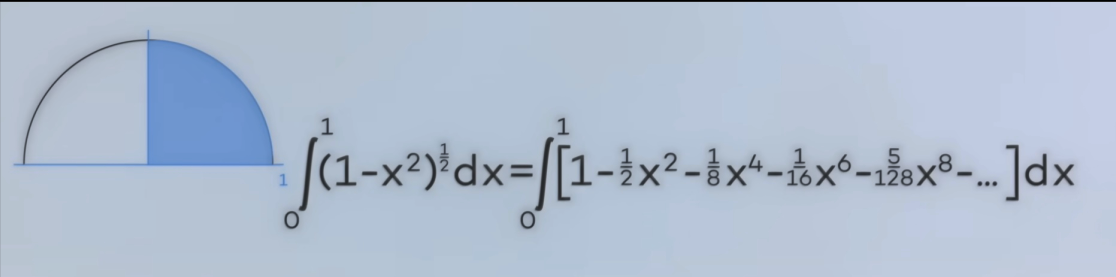
\includegraphics[width=0.5\linewidth]{fig/Area_del_circulo.png}
\end{center}

\noindent \textbf{SÓCRATES:} ¡Por suerte, Newton acababa de inventar el
cálculo! Entonces, ¿de qué otra forma podría calcular el área bajo esta
curva?

\noindent \textbf{SIMPLICIO:} ¡Con una integral! Así que:
\[ \frac{\pi}{4} = \int_{0}^{1} \sqrt{1 - x^2} \, dx = \int_{0}^{1} \left( 1 - \frac{x^2}{2} - \frac{x^4}{8} - \frac{x^6}{16} - \frac{5x^8}{128} - \dots \right) dx \]
Simplemente integraré término a término...

\noindent \textbf{SÓCRATES:} ¡Epa, espera un momento! ¿Por qué se te
permite...? Sabes qué, da igual, lo siento. Adelante.

\noindent \textbf{SIMPLICIO:} Qué raro eres. En fin. Integrando término
a término obtengo:
\[ \frac{\pi}{4} = \left[ x - \frac{x^3}{6} - \frac{x^5}{40} - \frac{x^7}{112} - \frac{5x^9}{1152} - \dots \right]_{0}^{1} \]
\[ = 1 - \frac{1}{6} - \frac{1}{40} - \frac{1}{112} - \frac{5}{1152} - \dots \]
¡Vaya! ¡Así que Newton obtuvo una serie infinita para $\pi$! Si evalúo solo estos cinco términos y multiplico por 4, obtengo la fracción $32057/10080 \approx 3,180$. ¡No está mal!

\noindent \textbf{SÓCRATES:} No está mal, en efecto. Sabes, Simplicio,
muchos artículos de matemáticas tienen prácticamente cero ideas nuevas;
simplemente hacen algo que nadie se molestó en hacer antes en un
contexto ligeramente distinto. Un artículo de matemáticas realmente
bueno puede tener una o dos ideas genuinamente nuevas. ¡Newton ya va por
la idea nueva número cinco, y aún no ha terminado!

\noindent \textbf{SIMPLICIO:} Vale, ¿y cuál es la idea nueva número
seis?

\noindent \textbf{SÓCRATES:} Bueno, ¿recuerdas que integraste hasta
$x = 1$? En tu serie,
\[ \frac{\pi}{4} = \left[ x - \frac{x^3}{6} - \frac{x^5}{40} - \frac{x^7}{112} - \frac{5x^9}{1152} - \dots \right]_{0}^{1} \]
tienes todas estas potencias altas de $x$, pero se están
``desperdiciando'' porque estás poniendo $x = 1$. ¿Y si en su lugar solo
integraras hasta, por ejemplo, $x = 1/2$?

\noindent \textbf{SIMPLICIO:} ¡Ah, qué guay! Entonces la serie
convergerá mucho más rápido. Pero espera, eso cambia la geometría. En
lugar de un cuarto de círculo, ahora tenemos... un sector de 30 grados,
que tiene un área de $\pi/12$, más un triángulo 30-60-90 (¡ah, por eso
sugeriste $x = 1/2$!) con área
$\frac{1}{2} \times \frac{1}{2} \times \frac{\sqrt{3}}{2}$.

\begin{center}
    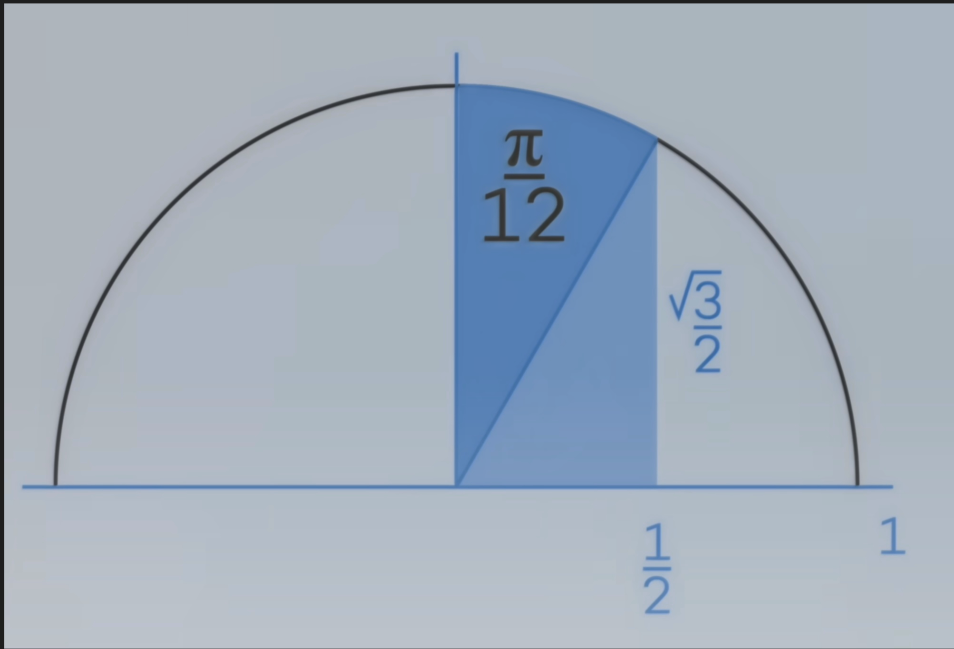
\includegraphics[width=0.5\linewidth]{fig/Circulo_sector_y_triangulo.png}
\end{center}

\noindent ¡Menos mal que ya sabemos cómo estimar $\sqrt{3}$ rápidamente
con gran precisión! (Esa es la contrapartida: podríamos elegir una $x$
aún más pequeña para una convergencia más rápida, pero entonces
tendríamos que lidiar con evaluaciones geométricas cada vez más
complicadas; así que $x = 1/2$ es el ``punto ideal''). Así que ahora:
\[ \frac{\pi}{12} + \frac{\sqrt{3}}{8} = \left[ x - \frac{x^3}{6} - \frac{x^5}{40} - \frac{x^7}{112} - \frac{5x^9}{1152} - \dots \right]_{0}^{1/2} \]
\[ = \frac{1}{2} - \frac{1}{6} \left(\frac{1}{2}\right)^3 - \frac{1}{40} \left(\frac{1}{2}\right)^5 - \frac{1}{112} \left(\frac{1}{2}\right)^7 - \frac{5}{1152} \left(\frac{1}{2}\right)^9 - \dots \]
Evaluando de nuevo solo estos cinco términos obtenemos la fracción
$9874097/20643840$. Y ahora, aislando $\pi$ obtenemos la estimación:
\[ \pi \approx 12 \times \left( 9874097/20643840 - \frac{\sqrt{3}}{8} \right) \approx 3,14161, \]
que solo difiere en dos partes por cada 100.000 de la estimación real $\pi
\approx 3,14159$. ¡Y todo eso con solo cinco términos, increíble!

\noindent \textbf{SÓCRATES:} Sí, Newton fue realmente
impresionante. Aquí tienes un buen vídeo de YouTube de Veritasium que
analiza toda esta saga: \url{https://youtu.be/gMlf1ELvRzc}

\noindent De hecho, una serie para $\pi$ similar a esta fue descubierta
dos siglos antes por el matemático indio Madhava de Sangamagrama. Y
harían falta dos siglos más hasta que los matemáticos descubrieran cómo
justificar rigurosamente el trabajo de Newton. Para hacerlo, tuvieron
que averiguar:
\begin{itemize}
\item ¿Qué significa que una sucesión de números reales
  $a_0, a_1, a_2, \dots$ converja?
\item ¿Qué significa que una serie (es decir, una sucesión de sumas
  parciales) $a_0 + a_1 + a_2 + \dots$ converja, y podríamos sumar estos
  números en cualquier orden que quisiéramos?
\item ¿Qué significa que una serie que involucra una variable, como una
  serie de potencias $a_0 + a_1x + a_2x^2 + \dots$, converja, y si es
  así, a qué tipo de función converge?
    \item ¿Cuándo podemos intercambiar límites con integrales, como al integrar término a término?
    \[ \int (a_0 + a_1x + a_2x^2 + \dots) dx \stackrel{?}{=} \int a_0 dx + \int a_1x dx + \int a_2x^2 dx + \dots \]
\end{itemize}
Etcétera, etcétera. ¡Tenemos mucho trabajo por hacer!

\noindent \textbf{SIMPLICIO:} Vale, vale; ¡me has convencido! Empecemos
con algo de análisis real de verdad, por favor.

\section{La definición principal}

Nuestro primer paso para dar rigor al argumento de Newton es deletrear
exactamente qué queremos decir cuando una sucesión $a_n$
converge. Costará un poco de trabajo construir la definición y, lo que
es más importante, entender \textit{por qué} parece una definición
razonable.

Pero primero: por alguna razón (probablemente la culpa sea de Euler),
las matemáticas tienen dos convenciones completamente diferentes para
escribir funciones. Para funciones generales
$f : \mathbb{R} \to \mathbb{R}$, escribimos $f(x)$, con paréntesis. Pero cuando trabajamos
con sucesiones, $a_n$, es decir, $a_0, a_1, a_2, \dots$, cambiamos
extrañamente a subíndices. ¿Por qué? Accidente histórico.

Una sucesión no es más que una función cuyo ``dominio'' (es decir, el
conjunto de entradas a la función) son los números naturales; así que
romperemos con la tradición y unificaremos las dos convenciones,
escribiendo de ahora en adelante $a : \mathbb{N} \to \mathbb{R}$ para sucesiones de números
reales, $a(0), a(1), a(2), \dots$.

Ahora bien, la definición que los matemáticos acabaron creando para lo
que significa que una sucesión converja era tan intrincada (al menos a
primera vista) ¡que tuvo que ser inventada dos veces!

La formulación final cristalizó a través del trabajo de Karl Weierstrass
en la década de 1860, quien transformó el análisis de un arte intuitivo
en una ciencia rigurosa. Sin embargo, las semillas de esta idea
aparecieron mucho antes en el trabajo de Bernard Bolzano. En las décadas
de 1810 y 1820, Bolzano estaba desarrollando ideas asombrosamente
modernas sobre la continuidad y los límites, pero estaba demasiado
adelantado a su tiempo para que la comunidad matemática aceptara estos
conceptos abstractos. Solo en la época de Weierstrass —medio siglo
después— calaron estas ideas.

Sin más preámbulos, aquí está:

\begin{definicion}[Convergencia de sucesiones]
  Dada una sucesión $a : \mathbb{N} \to \mathbb{R}$ y un número real
  $L : \mathbb{R}$, escribimos $\lim a = L$ y decimos que la sucesión
  $a$ \textbf{converge} a $L$, si: para cada $\varepsilon > 0$, existe un
  $N \in \mathbb{N}$ tal que, para todo $n \geq N$, tenemos $|a(n) - L| < \varepsilon$.
\end{definicion}

Esta definición probablemente no sea la primera, ni la segunda, ni la
décima cosa que se te habría ocurrido. Pero con el tiempo, espero que
llegues a ver que encarna una hermosa negociación entre precisión y
esfuerzo.

Me gusta pensar en ello como una conversación entre un ingeniero y un
maquinista. El ingeniero llega con las especificaciones: ``Vamos a
fabricar esta pieza, y necesito que su longitud sea de 1 pie, con una
tolerancia de error de 1/100 de pulgada''.

El maquinista responde: ``Claro, puedo hacerlo, pero tendré que hacer
funcionar mi equipo especial durante al menos 10 horas para garantizar
esa tolerancia''. El ingeniero responde: ``Lo siento, me equivoqué,
¿podemos cambiar la tolerancia a 1/1000 de pulgada?''. El maquinista
responde: ``Uf, sí, podemos hacerlo, pero te costará. Necesitaré al
menos 40 horas de operación, pero después de eso, te lo garantizo''.

Mientras esta conversación pueda continuar independientemente de
\textit{cualquier} tolerancia $\varepsilon > 0$ que requiera el ingeniero, siendo
el maquinista siempre capaz de responder con un número mínimo finito de
horas $N$, tras el cual se alcanzará la tolerancia, podemos decir que el
equipo \textbf{converge}.

Leamos ahora la definición de Weierstrass (¿o es la de Bolzano?) otra
vez. Tenemos algún proceso que en el tiempo $n$ devuelve una lectura
$a(n)$ (piensa: longitud de la pieza). Nuestro objetivo final es
conseguir la longitud $L$. Si para cualquier tolerancia
$\varepsilon > 0$, por pequeña que sea, siempre existe algún tiempo mínimo
$N$, de modo que, para cualquier tiempo futuro $n \geq N$, se garantiza que
estaremos dentro de esa tolerancia, $|a(n) - L| < \varepsilon$, esa es exactamente
la condición bajo la cual diremos que la sucesión $a(n)$
\textbf{converge} a $L$.

\begin{center}
    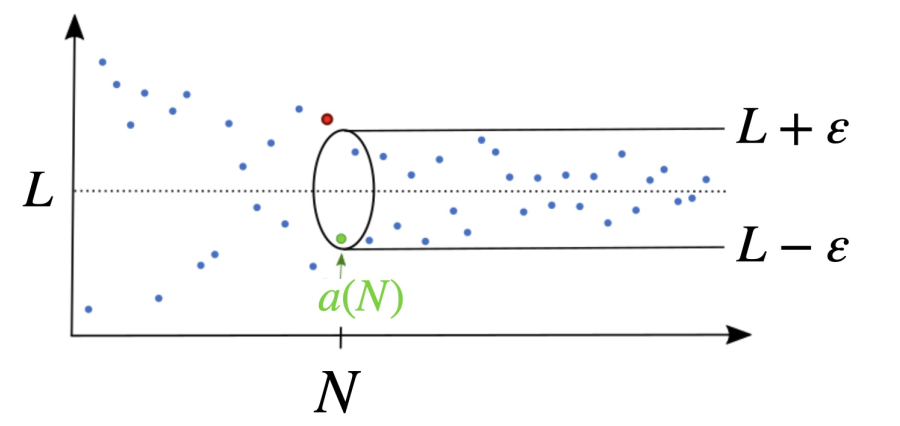
\includegraphics[width=0.5\linewidth]{fig/Convergencia.png}
\end{center}

Lo que hace que esta definición sea tan poderosa es su universalidad. El
maquinista está esencialmente prometiendo: ``Dame cualquier requisito de
tolerancia, por estricto que sea, y puedo cumplirlo, aunque necesite más
recursos (un $N$ mayor) para especificaciones más ajustadas''.

Fíjate en algo más sobre la definición: no hace mención a que algo
suceda ``eventualmente'', o ``en el infinito'' ni ninguna otra palabra
ambigua y escurridiza. Hemos cambiado la ambigüedad de hablar del
infinito por la precisión de los cuantificadores existenciales y
universales. No más imprecisiones sobre lo que sucede ``cuando $n$ se
hace grande''; en su lugar, tenemos un desafío concreto: dada cualquier
tolerancia $\varepsilon$, ¿puedes encontrar un umbral específico $N$? Esa idea fue
el avance clave que permitió que el Cálculo entrara en el reino de las
matemáticas rigurosas.

En Lean, la definición se escribe así:

\begin{minted}{lean}
def LimSuc (a : ℕ → ℝ) (L : ℝ) : Prop :=
  ∀ ε > 0, ∃ N : ℕ, ∀ n ≥ N, |a n - L| < ε
\end{minted}

Esta sintaxis debería resultarte familiar por la táctica \texttt{have}
que ya conoces. El símbolo especial \texttt{def} (en lugar de
\texttt{have}) significa que estamos a punto de definir algo, y
\texttt{LimSuc} es su nombre (por \textit{límite de sucesión}, por
supuesto; pero podríamos haberlo llamado como quisiéramos). Luego
nuestras suposiciones son una sucesión \texttt{a : N -> R} y algún
número real \texttt{L \in R}. Después de los dos puntos \texttt{:} va
nuestra salida, que en este caso es \texttt{Prop}, es decir, una
proposición (sentencia) que puede ser verdadera o falsa. Así que
\texttt{LimSuc} es en realidad una función que toma una sucesión y un
hipotético valor límite, y devuelve verdadero o falso dependiendo de si
se cumple la condición. Luego viene un signo de dos puntos e igual
\texttt{:=}, tras el cual se especifica la condición exacta que se va a
probar. Y la condición es lo que ya dijimos: para todo epsilon, .... La
gran diferencia es que puedes escribir \texttt{have} dentro de una
demostración, pero no puedes escribir \texttt{def} dentro de una;
\texttt{def} está reservado para crear definiciones globales a las que
se puede hacer referencia para siempre una vez introducidas.

Puede que te resulte útil una nueva táctica llamada \texttt{change}. Te
permite reemplazar un objetivo (o hipótesis) por algo que es
definicionalmente igual a él. En nuestro ejemplo, verás el objetivo como
\texttt{LimSuc a L}. ¿Qué se supone que debes hacer con eso? Bueno, si
recuerdas cómo se define \texttt{LimSuc}, entonces puedes reemplazar el
objetivo con la definición, escribiendo:

\begin{minted}{lean}
change ∀ ε > 0 , ∃ N : ℕ, ∀ n ≥ N , |a n - L| < ε
\end{minted}

Lean cambiará entonces el objetivo por su definición. Recuerda que
$\varepsilon, N$ y $n$ son todas variables mudas aquí, así que puedes divertirte
un poco:

\begin{minted}{lean}
change ∀ Alicia > 0 , ∃ Bob : ℕ, ∀ Blas ≥ Bob , |a Blas - L| < Alicia
\end{minted}

Y una última táctica que también podrías encontrar útil es
\texttt{norm\_num} (para normalizar valores numéricos); evalúa
expresiones numéricas y demuestra igualdades/desigualdades que
involucren números concretos. Por ejemplo, si te quedas atascado con un
$|0|$ en algún momento y quieres convertirlo en un simple $0$, intenta
llamar a \texttt{norm\_num}.

\begin{minted}{lean}
-- ---------------------------------------------------------------------
-- Demostrar que si a es una sucesión tal que para todo
-- n, a(n) = L, entonces a converge a L.
-- ----------------------------------------------------------------------

-- Demostración en lenguaje natural
-- ================================

-- Tenemos que demostrar que para cada ε ∈ ℝ tal que ε > 0, existe un
-- N ∈ ℕ, tal que (∀n ∈ ℕ)[n ≥ N → |a(n) - L| < ε]. Basta tomar N como
-- 0, ya que para todo n ≥ N se tiene
--    |a(n) - L| = |L - L|
--               = |0|
--               = 0
--               < ε

-- Demostraciones con Lean4
-- ========================

variable (a : ℕ → ℝ)
variable (L : ℝ)

-- 1ª demostración
-- ===============

example
  (h : ∀ n, a n = L)
  : LimSuc a L :=
by
  change ∀ ε > 0 , ∃ N : ℕ, ∀ n ≥ N , |a n - L| < ε
  -- ⊢ ∀ ε > 0, ∃ N, ∀ n ≥ N, |a n - L| < ε
  intro ε hε
  -- ε : ℝ
  -- hε : ε > 0
  -- ⊢ ∃ N, ∀ n ≥ N, |a n - L| < ε
  use 0
  -- ⊢ ∀ n ≥ 0, |a n - L| < ε
  intro n hn
  -- n : ℕ
  -- hn : n ≥ 0
  -- ⊢ |a n - L| < ε
  specialize h n
  -- h : a n = L
  rewrite [h]
  -- ⊢ |L - L| < ε
  ring_nf
  -- ⊢ |0| < ε
  norm_num
  -- ⊢ 0 < ε
  exact hε

-- 2ª demostración
-- ===============

example
  (h : ∀ n, a n = L)
  : LimSuc a L :=
by
  intros ε hε
  -- ε : ℝ
  -- hε : ε > 0
  -- ⊢ ∃ N, ∀ (n : ℕ), n ≥ N → |a n - L| < ε
  use 0
  -- ⊢ ∀ (n : ℕ), n ≥ 0 → |a n - L| < ε
  intros n hn
  -- n : ℕ
  -- hn : n ≥ 0
  -- ⊢ |a n - L| < ε
  show |a n - L| < ε
  calc |a n - L| = |L - L| := by rw [h n]
               _ = |0|     := by {congr ; exact sub_self L}
               _ = 0       := abs_zero
               _ < ε       := hε

-- 3ª demostración
-- ===============

example
  (h : ∀ n, a n = L)
  : LimSuc a L :=
by
  intros ε hε
  -- ε : ℝ
  -- hε : ε > 0
  -- ⊢ ∃ N, ∀ (n : ℕ), n ≥ N → |a n - L| < ε
  use 0
  -- ⊢ ∀ (n : ℕ), n ≥ 0 → |a n - L| < ε
  intros n hn
  -- n : ℕ
  -- hn : n ≥ 0
  -- ⊢ |a n - L| < ε
  show |a n - L| < ε
  calc |a n - L| = 0 := by simp [h n]
               _ < ε := hε

-- 4ª demostración
-- ===============

example
  (h : ∀ n, a n = L)
  : LimSuc a L :=
by
  intros ε hε
  -- ε : ℝ
  -- hε : ε > 0
  -- ⊢ ∃ N, ∀ (n : ℕ), n ≥ N → |a n - L| < ε
  aesop

-- 5ª demostración
-- ===============

example
  (h : ∀ n, a n = L)
  : LimSuc a L :=
by
  intros ε hε
  -- ε : ℝ
  -- hε : ε > 0
  -- ⊢ ∃ N, ∀ (n : ℕ), n ≥ N → |a n - L| < ε
  aesop

-- 6ª demostración
-- ===============

example
  (h : ∀ n, a n = L)
  : LimSuc a L :=
fun ε hε ↦ by aesop

-- Lemas usados
-- ============

#check (sub_self a : a - a = 0)
\end{minted}

¡Acabas de completar tu primera demostración rigurosa de un límite!
Reflexionemos sobre lo que has logrado y las ideas clave de este ejemplo
fundacional.

\textbf{Lo que acabas de demostrar:} Has demostrado que si una sucesión
siempre devuelve el mismo valor $L$, entonces converge a $L$. La
respuesta del maquinista a cualquier demanda de tolerancia
$\varepsilon > 0$ es bellamente simple: ``¡Puedo cumplir esa especificación
inmediatamente con cualquier longitud de producción $N$, porque ya estoy
produciendo exactamente lo que quieres!''.

\textbf{Ideas clave de esta demostración:}
\begin{enumerate}
\item \textbf{La táctica \texttt{change}:} Aprendiste a desplegar una
  definición para ver qué es lo que realmente estás intentando
  demostrar. \texttt{LimSuc a L} se convirtió en la condición concreta
  epsilon--$N$.
\item \textbf{La estructura lógica:} La demostración siguió el flujo
  natural de la definición:
    \begin{itemize}
    \item \texttt{intro \epsilon\ h\epsilon} manejó el ``para todo $\varepsilon > 0$''.
    \item \texttt{use 1} proporcionó el testigo $N$ (¡cualquier número
      sirve!).
    \item \texttt{intro n hn} manejó el ``para todo $n \geq N$''.
    \item Luego la manipulación algebraica mostró que
      $|a(n) - L| = |L - L| = |0|$.
    \item Después, la normalización numérica dio que $|0| = 0$, y
      \texttt{h\epsilon} finalmente demostró que $0 < \varepsilon$.
    \end{itemize}
\end{enumerate}

\textbf{La hermosa simplicidad:} Este es el escenario soñado por el
maquinista: no importa cuán exigentes sean los requisitos de tolerancia
del ingeniero, la fábrica de constantes puede satisfacerlos
instantáneamente. ¡No hay compromiso entre precisión y esfuerzo porque
el resultado ya es perfecto!

Estás construyendo la base de todo el cálculo. Cada límite, derivada e
integral descansa en última instancia en argumentos como este.


Alejémonos un poco de la demostración formal de Lean y entendamos qué
acabamos de demostrar en lenguaje natural.

\begin{theorem}
  Si una sucesión tiene el mismo valor para cada término, entonces
  converge a ese valor constante.
\end{theorem}

\begin{proof}
  Supongamos que tenemos una sucesión $a(n)$ donde $a(n) = L$ para todo
  $n$, y queremos demostrar que esta sucesión converge a $L$.

  Por definición, necesitamos demostrar que para cualquier tolerancia
  $\varepsilon > 0$, podemos encontrar un punto $N$ tal que para todo
  $n \geq N$, tenemos $|a(n) - L| < \varepsilon$.

  Esto es casi trivialmente simple: como $a(n) = L$ para cada $n$,
  tenemos:
  \[ |a(n) - L| = |L - L| = |0| = 0 \]
  Como $0 < \varepsilon$ para cualquier $\varepsilon$ positivo, podemos elegir cualquier
  $N$ que queramos (elegimos $N = 1$ en la demostración, pero $N = 0$ o
  $N = 1000$ funcionarían igual de bien).

  Por lo tanto, para cualquier $n \geq N$, tenemos
  $|a(n) - L| = 0 < \varepsilon$, lo que demuestra la convergencia.
\end{proof}


%%% Local Variables:
%%% mode: LaTeX
%%% TeX-master: "Analisis_en_Lean"
%%% End:
